\documentclass[12pt]{article}
\usepackage{times} 			% use Times New Roman font

\usepackage[margin=1in]{geometry}   % sets 1 inch margins on all sides
\usepackage{hyperref}               % for URL formatting
\usepackage[pdftex]{graphicx}       % So includegraphics will work
\setlength{\parskip}{1em}           % skip 1em between paragraphs
\usepackage{indentfirst}            % indent the first line of each paragraph
\usepackage{datetime}
\usepackage[small, bf]{caption}
\usepackage{listings}               % for code listings
\usepackage{xcolor}                 % for styling code
\usepackage{multirow}

\usepackage{float}

%New colors defined below
\definecolor{backcolour}{RGB}{246, 246, 246}   % 0xF6, 0xF6, 0xF6
\definecolor{codegreen}{RGB}{16, 124, 2}       % 0x10, 0x7C, 0x02
\definecolor{codepurple}{RGB}{170, 0, 217}     % 0xAA, 0x00, 0xD9
\definecolor{codered}{RGB}{154, 0, 18}         % 0x9A, 0x00, 0x12

%Code listing style named "gcolabstyle" - matches Google Colab
\lstdefinestyle{gcolabstyle}{
  basicstyle=\ttfamily\small,
  backgroundcolor=\color{backcolour},   
  commentstyle=\itshape\color{codegreen},
  keywordstyle=\color{codepurple},
  stringstyle=\color{codered},
  numberstyle=\ttfamily\footnotesize\color{darkgray}, 
  breakatwhitespace=false,         
  breaklines=true,                 
  captionpos=b,                    
  keepspaces=true,                 
  numbers=left,                    
  numbersep=5pt,                  
  showspaces=false,                
  showstringspaces=false,
  showtabs=false,                  
  tabsize=2
}

\lstset{style=gcolabstyle}      %set gcolabstyle code listing

% to make long URIs break nicely
\makeatletter
\g@addto@macro{\UrlBreaks}{\UrlOrds}
\makeatother

% for fancy page headings
\usepackage{fancyhdr}
\setlength{\headheight}{13.6pt} % to remove fancyhdr warning
\pagestyle{fancy}
\fancyhf{}
\rhead{\small \thepage}
\lhead{\small HW4, Adeniran}  % EDIT THIS, REPLACE # with HW number
\chead{\small CS 532, Spring 2021} 

%-------------------------------------------------------------------------
\begin{document}

\begin{centering}
{\large\textbf{HW4 - Social Media}}\\ % EDIT THIS
                                % REPLACE # with HW num and ADD title
Adeniran Adeniyi\\                     % EDIT THIS
March 17th 11:59 PM\\                      % EDIT THIS
\end{centering}

%-------------------------------------------------------------------------

% The * after \section just says to not number the sections
%----------------------------Q1111111111111111111111111111111111

\section*{Q1}
\emph{Compute the mean, standard deviation, and median of the number of friends that the user's friends have.\\
Create a graph of the number of friends (y-axis) and the friends (x-axis) themselves, sorted by number of friends (y-axis). (The friends don't need to be labeled on the x-axis: just f1, f2, f3, ... fn.) Include the user in the graph (count the number of their friends) and label as U.}
\subsection*{\color{blue}{Answer}}
\lstinputlisting[language=Python,caption=friendPradox.py, label=Q1:import,firstnumber=1,firstline=1,lastline=40]{friendPradox.py}

\begin{figure}[H]
    \centering
    % trim and clip are used to crop the image, trim=left bottom right top
    % width sets max width, height will be scaled appropriately
    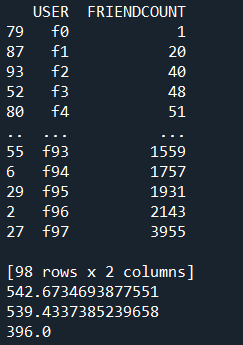
\includegraphics[trim=0 0 0 0, clip, width=\textwidth] {console_output1.PNG}
    \caption{Shows the pandas data and mean,std and meadian respectsively}
    \label{fig:Running output}
\end{figure}

\begin{figure}[H]
    \centering
    % trim and clip are used to crop the image, trim=left bottom right top
    % width sets max width, height will be scaled appropriately
    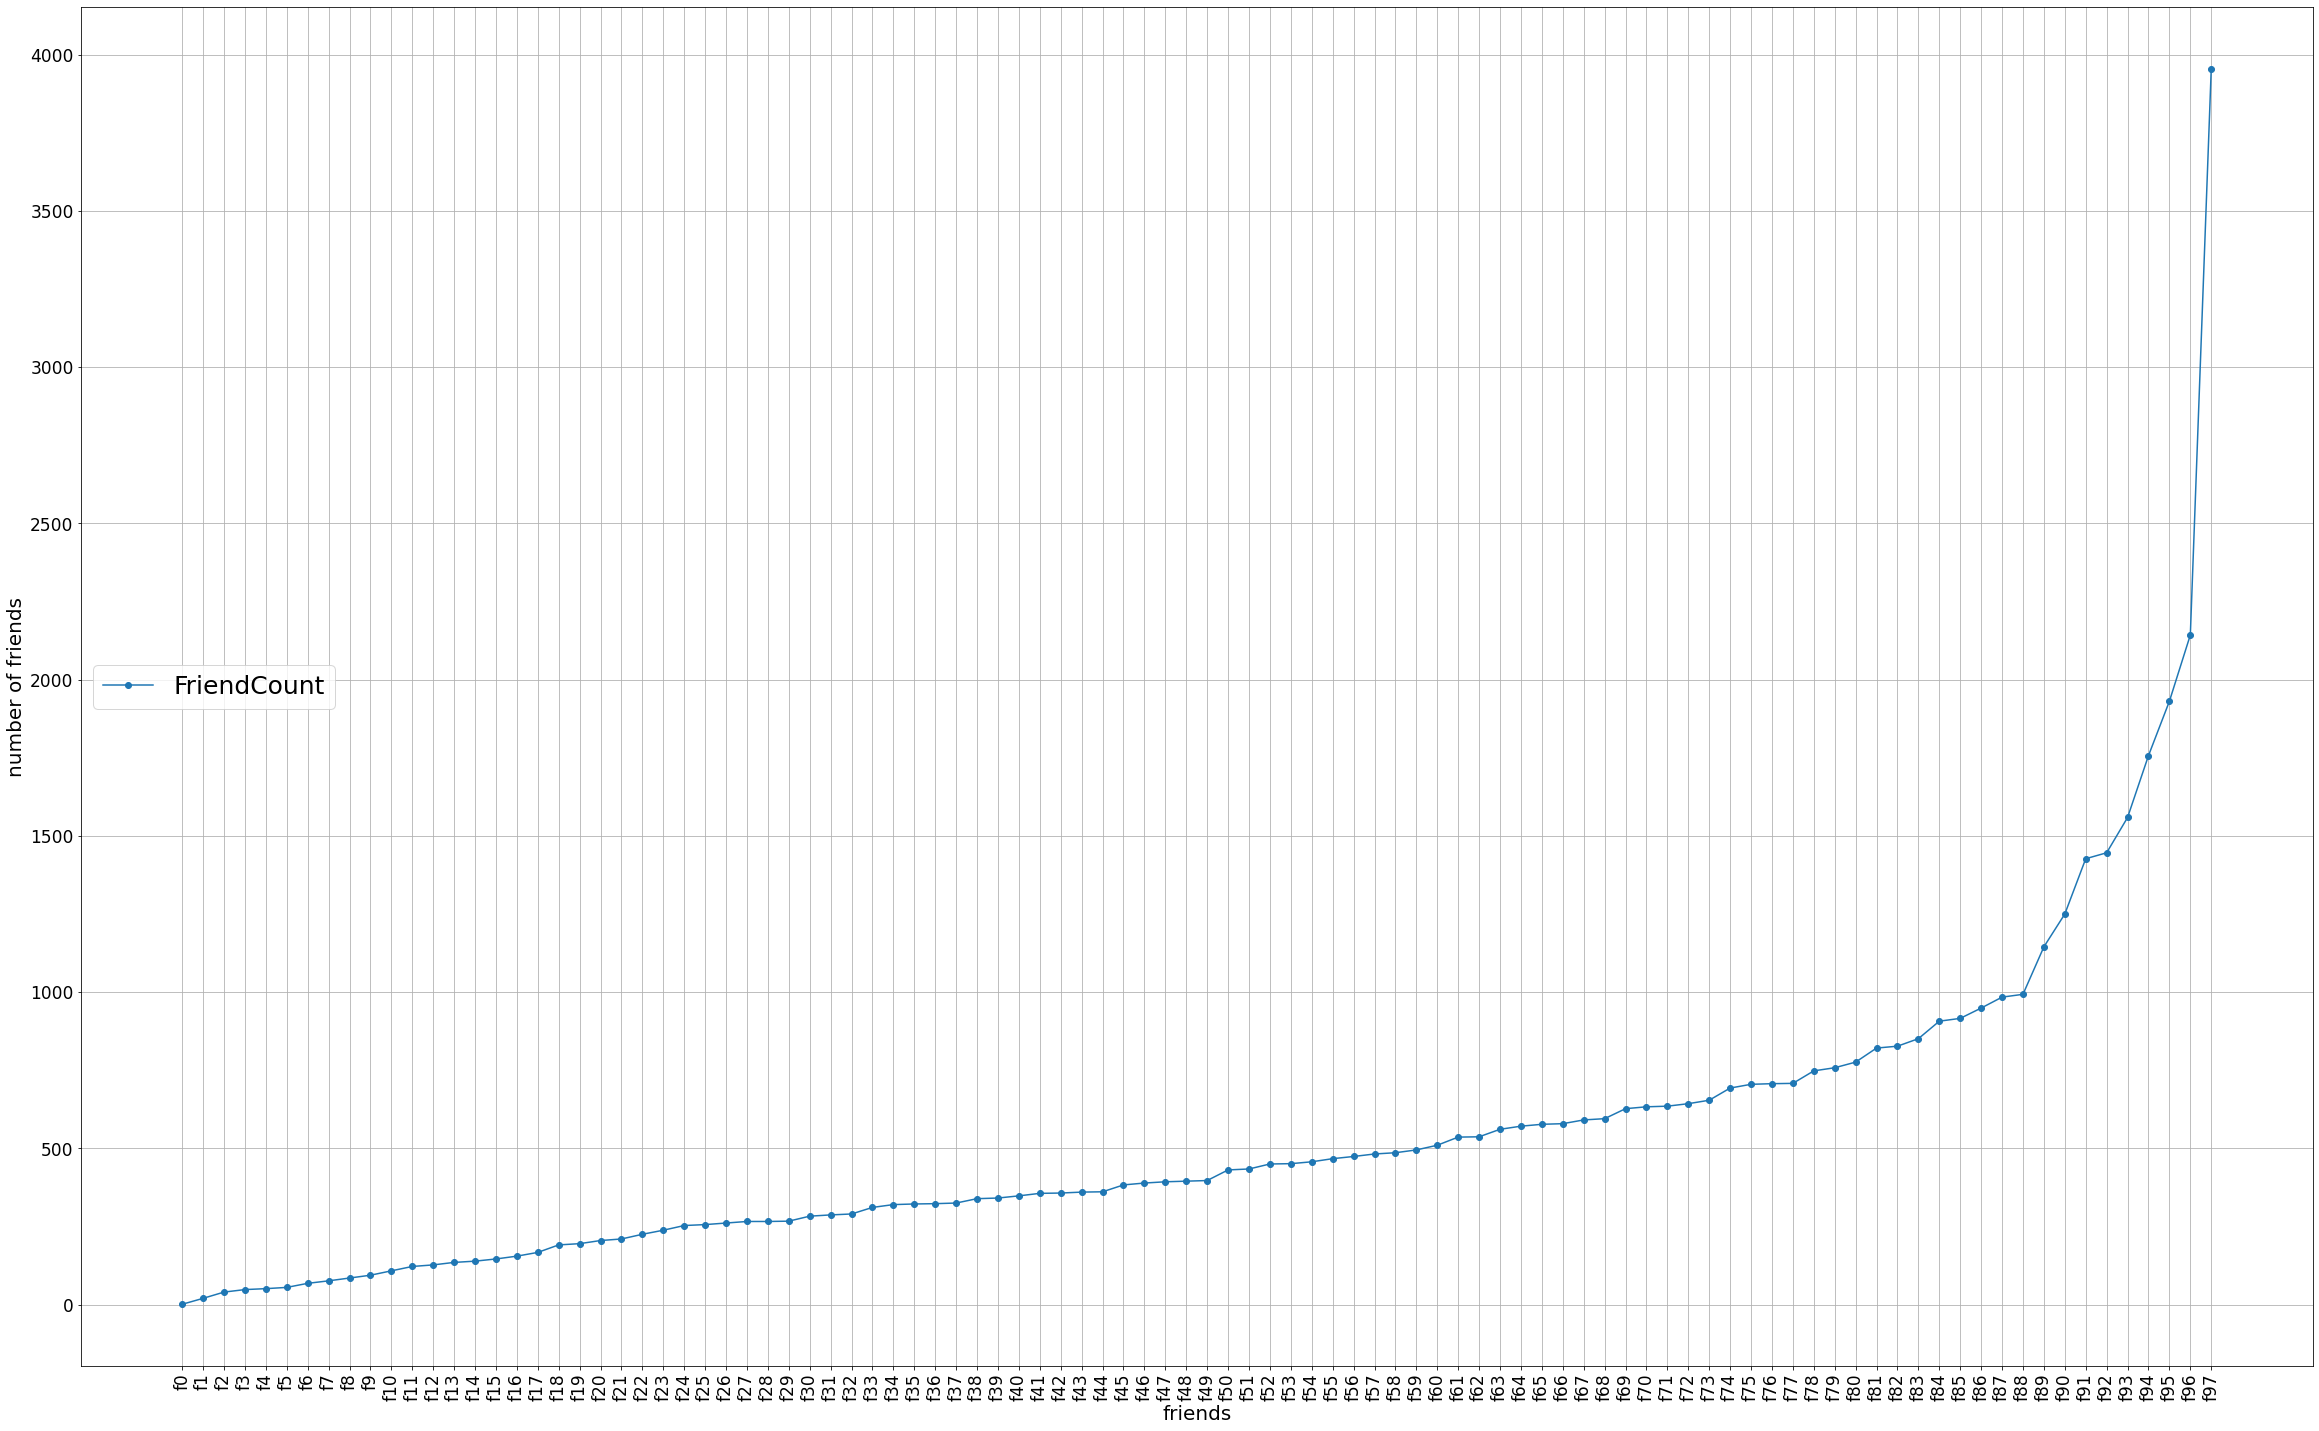
\includegraphics[trim=0 0 0 0, clip, width=\textwidth] {finalPotQ1.PNG}
    \caption{The plot for Q1 }
    \label{fig:q1}
\end{figure}
\subsection*{Discussion}
\emph{I followed these instruction below:}
    \begin{itemize}
        \item I read the csv file using the pandas library \begin{list}{$\circ$}
                \item Removed the extra space in the column head on line 14 of friendPradox.py
            \end{list}
        \item sorted the values of the FriendCount column
        \item constructed a list of f0, f1,f2 ,..., fn - iitems equal to the number of size of the data in pandas dataframe on line 19 - 24
        \item Replaced the User column in dataframe with the list values. on line 26
        \item Using the data frame built in function I was able to calculate:\\
        Mean to be: 542.67 \\
        Standard deviation:539.43 \\
        Median to be:396.0 
        
        \item finally plotted the graph in Figure \ref{fig:q1}
    \end{itemize}
\section*{Q2}
\emph{
Determine if the friendship paradox holds for your Twitter account. Since Twitter is a directed graph, use followers as the value you measure (i.e., "do your followers have more followers than you?"). Due to Twitter rate limits, this part will take some time to complete.
Generate the same graph as in Q1, and calculate sthe same mean, standard deviation, and median values.}
\subsection*{\color{blue}{Answer}}
\lstinputlisting[language=Python,caption=followerExtactor.py, label=Q1:import,firstnumber=1,firstline=1,lastline=152]{followerExtactor.py}
\begin{figure}[H]
\centering
% trim and clip are used to crop the image, trim=left bottom right top
% width sets max width, height will be scaled appropriately
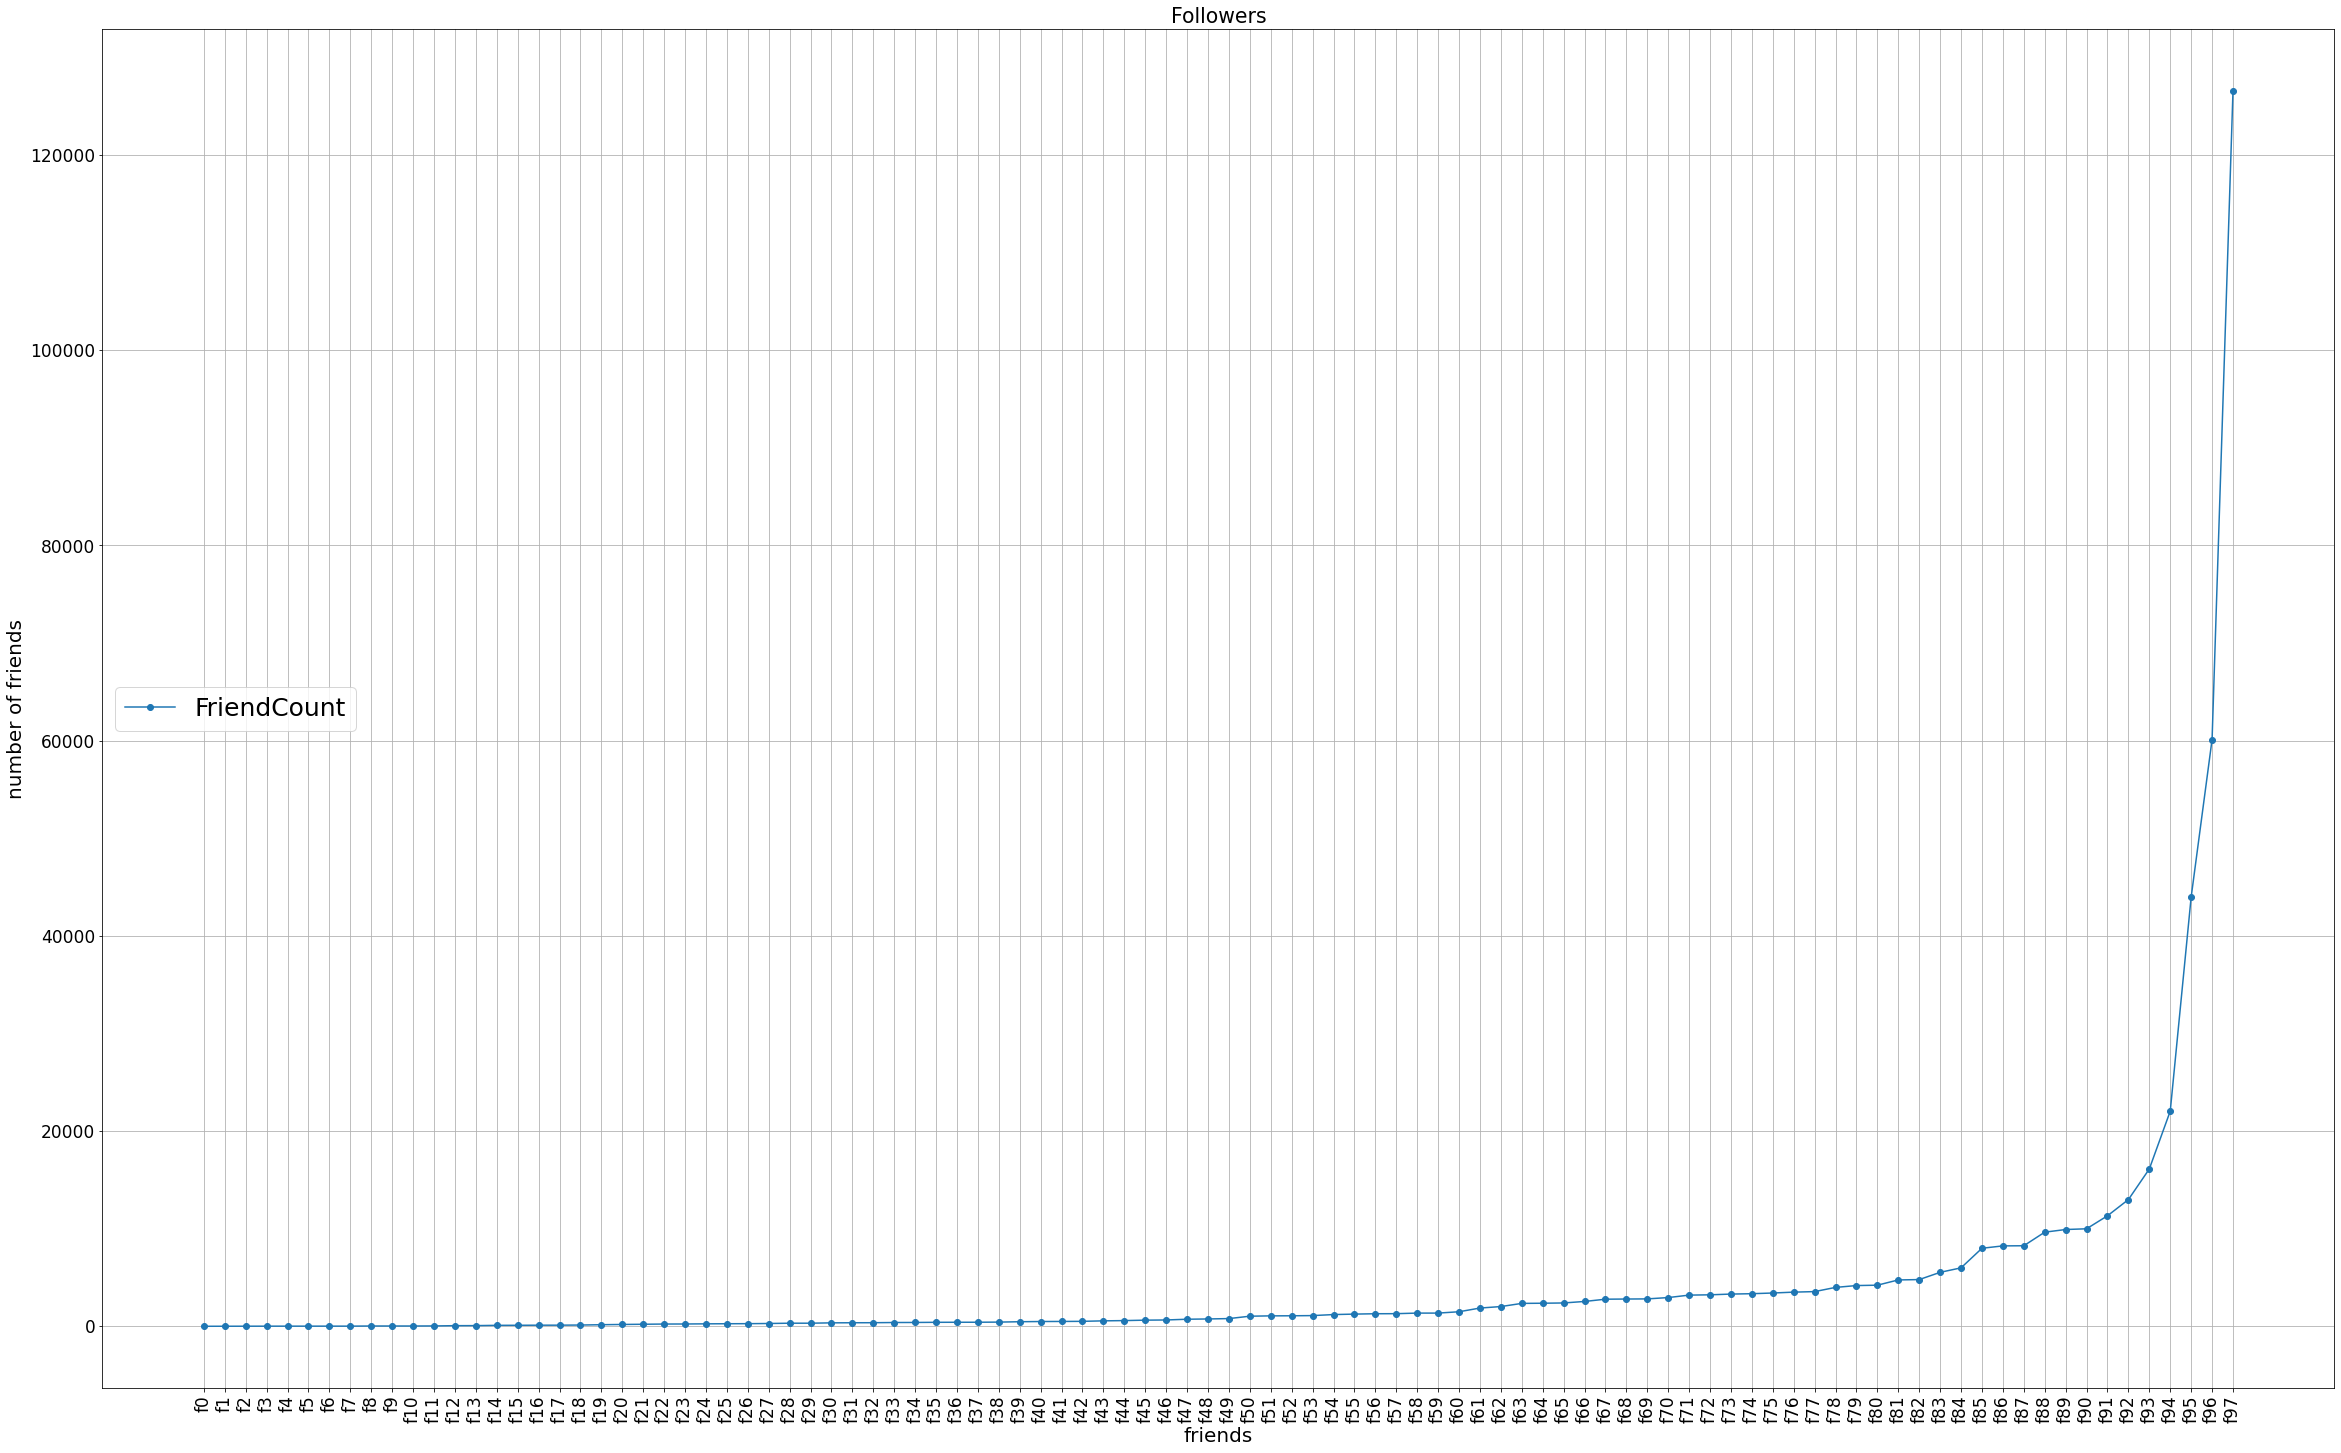
\includegraphics[trim=0 0 0 0, clip, width=\textwidth] {followers.PNG}
\caption{The plot for Q2 followers }
\label{fig:q2}
\end{figure}

\begin{figure}[H]
    \centering
    % trim and clip are used to crop the image, trim=left bottom right top
    % width sets max width, height will be scaled appropriately
    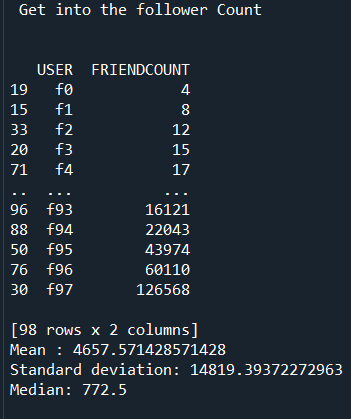
\includegraphics[trim=0 0 0 0, clip, width=\textwidth] {followers_console_out.png}
    \caption{shows the console output for Q2}
    \label{fig:Running output}
\end{figure}
\subsection*{Discussion}
\emph{I followed these instruction below:}
    \begin{itemize}
        \item I created a function called getUserFollowers in line 67 of followerExtractor.py \lstinputlisting[language=Python,caption=The function in followerExtractor.py, label=Q1:import,firstnumber=67,firstline=67,lastline=67]{followerExtactor.py}
            \begin{list}{$\circ$}
                \item Using my twiter account screen name(adeniran827),
                \lstinputlisting[language=Python,caption=Twitter name used in followerExtractor.py, label=Q1:import,firstnumber=114,firstline=114,lastline=114]{followerExtactor.py}
                \item  I retrived all of my followers ID (Limited this list to 98 on line 70 -71)
                \lstinputlisting[language=Python,caption=Using tweepy to store the list of my followers\,saved ids in p followerExtractor.py, label=Q1:import,firstnumber=70,firstline=70,lastline=71]{followerExtactor.py}
                \lstinputlisting[language=Python,caption=Limiting the list gotten from p in followerExtractor.py, label=Q1:import,firstnumber=79,firstline=79,lastline=80]{followerExtactor.py}
                \item I Passed each user Id i got to the get\_number\_of\_followers\_followings function. \\ This function returned followers count of the associated user Id\begin{list}{$\circ$}
                        \item In line 57 to  59, ensured that followers count was possible, since 0 was parsed into the function along with the id of the user
                         \lstinputlisting[language=Python,caption=Using follower\_count to get the total followers a user have in followerExtractor.py, label=Q1:import,firstnumber=52,firstline=52,lastline=59]{followerExtactor.py}
                    \end{list}
                \item Parsed the generated list of users and followers count as a pandas dataframe to handledPandasDF\_Replacement function
                \item Sort the data frame in handledPandasDF\_Replacement
                \item Performed silimar operation of Q1, replacing the names with f0, f1,f2 ,..., fn - names
                \item Got the dataframe at line 120 of followerExtractor.py
                \item Got values of: \\
                mean: 4657 followers for my followers followers count\\
                std:14819.39\\
                median:772.5
                \item finally plotted the graph in Figure \ref{fig:q2}
                \item  Comparing the mean of  my followers followers' count 4657 to my followers count of 234. Those that I follow  have a higher followers count than I do.
                \item Comparing the mean to my current twitter followers of 234,  the first 98 of those that follow me have a higher following than I do. 
            \end{list}
        
    \end{itemize}

\section*{Q3}
\subsection*{\color{blue}{Answer}}
\lstinputlisting[language=Python,caption=snapshot that shows the followings process in followerExtractor.py, label=Q1:import,firstnumber=134,firstline=134,lastline=147]{followerExtactor.py}
\begin{figure}[H]
\centering
% trim and clip are used to crop the image, trim=left bottom right top
% width sets max width, height will be scaled appropriately
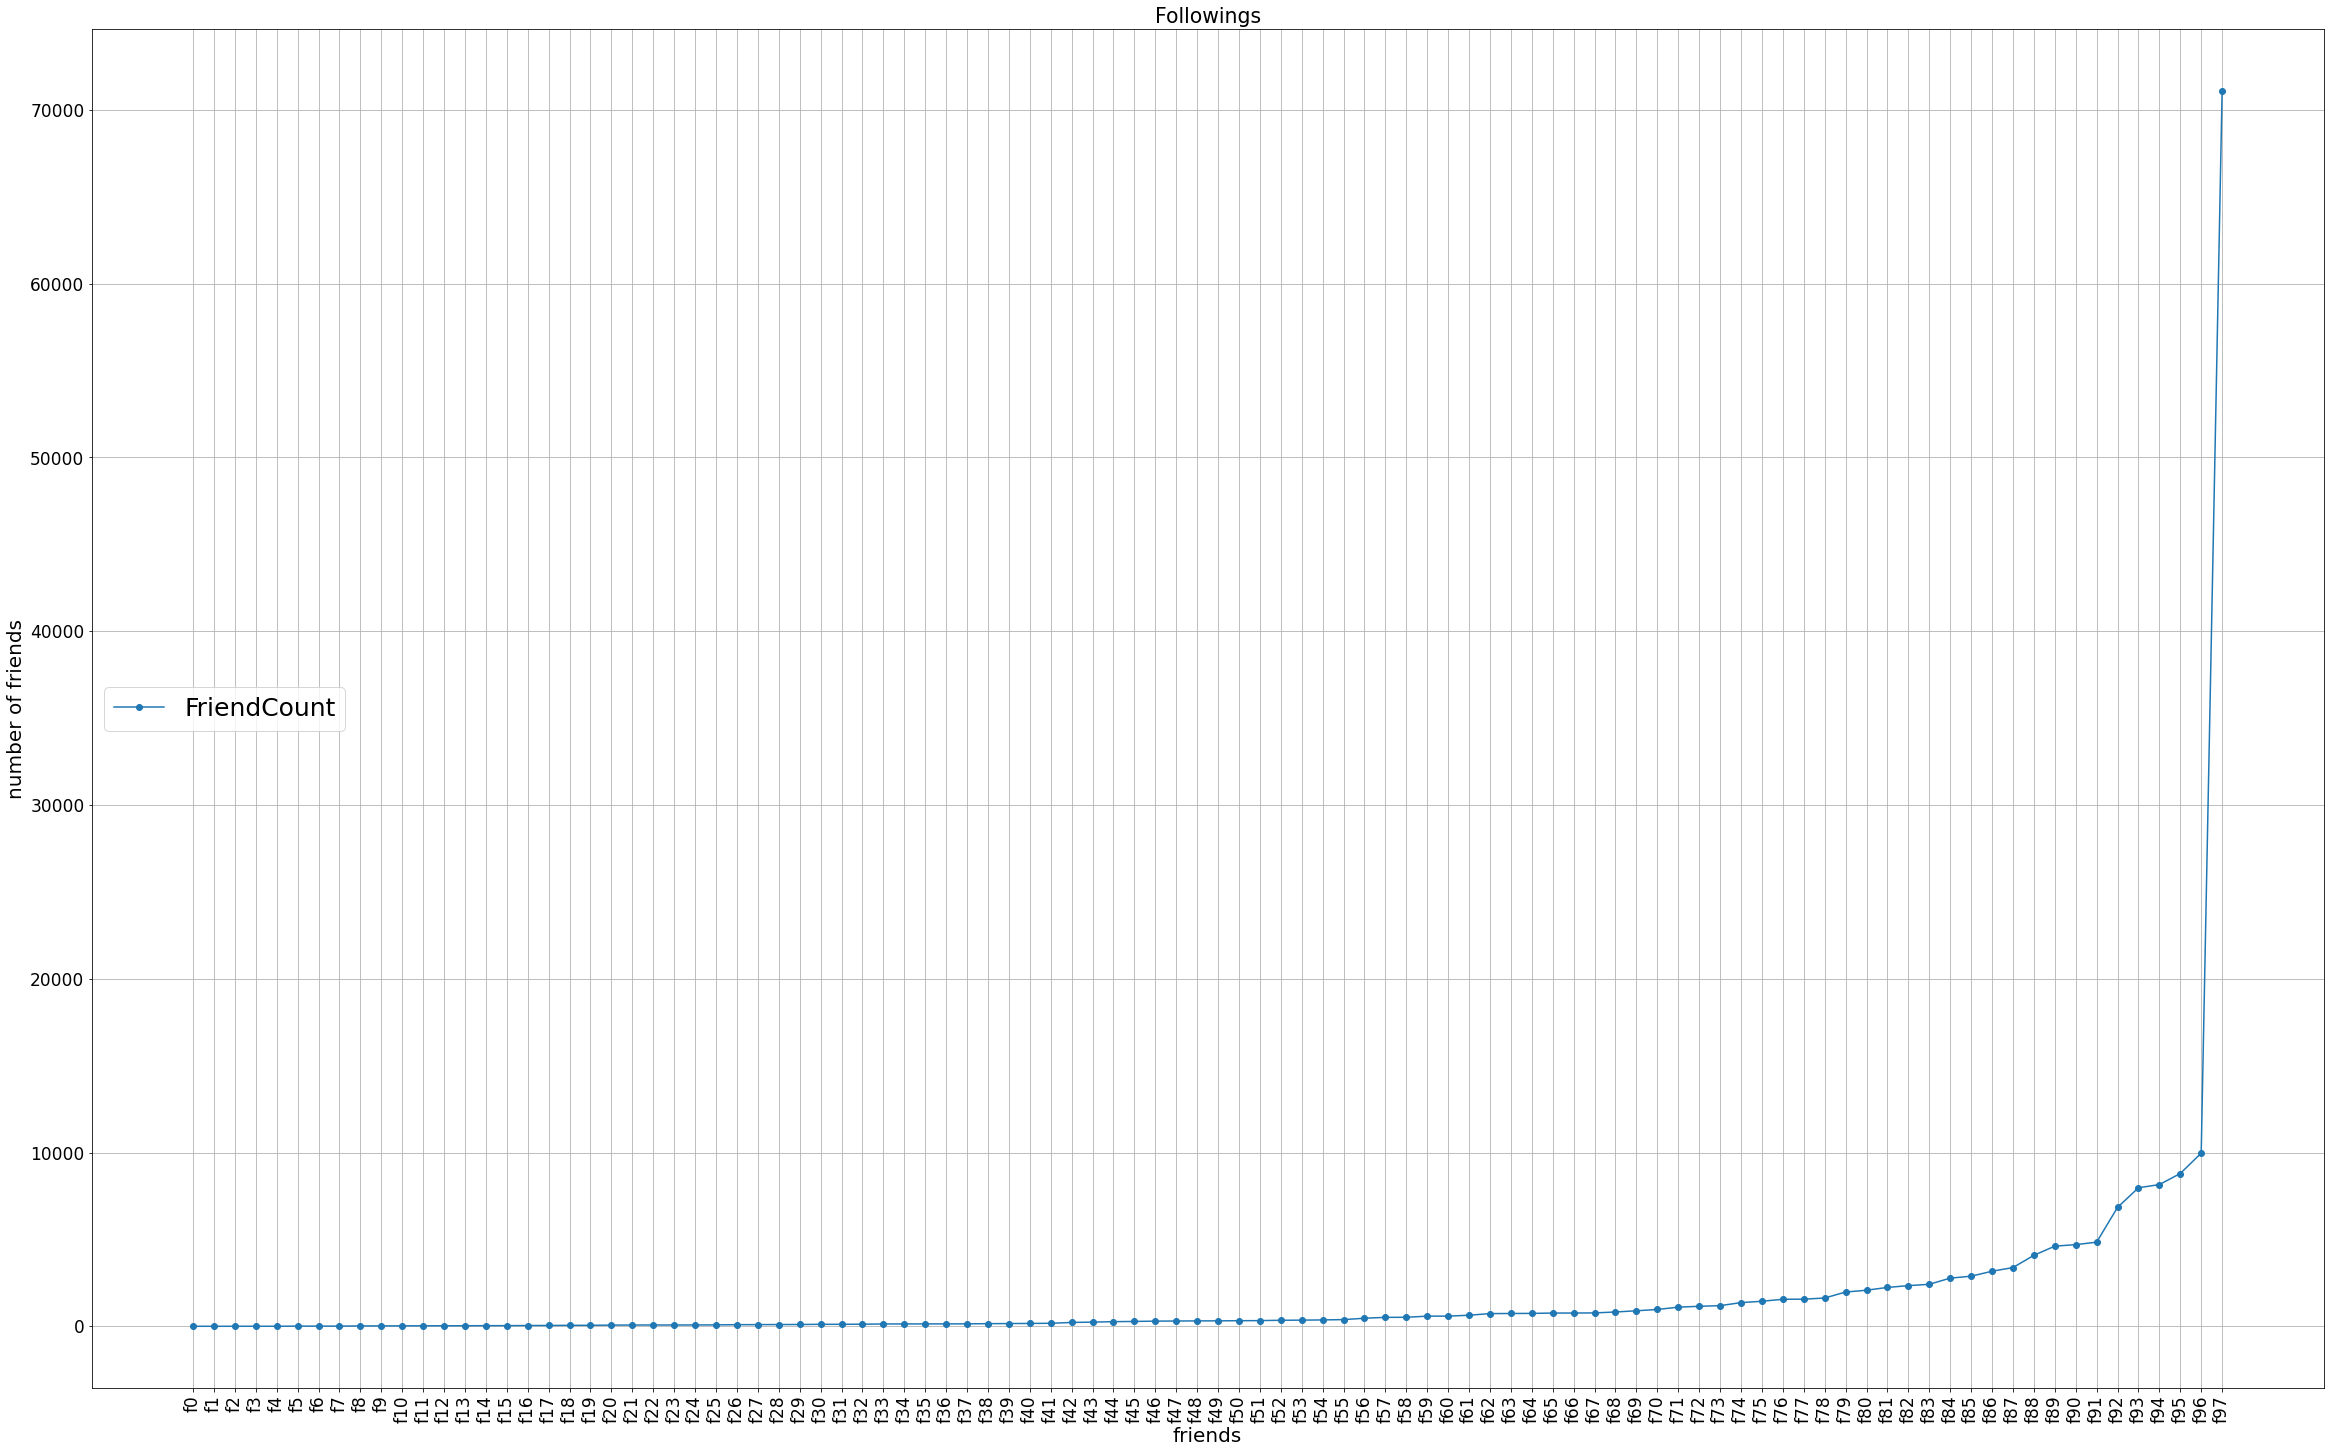
\includegraphics[trim=0 0 0 0, clip, width=\textwidth] {followings.PNG}
\caption{The plot for Q3 followings }
\label{fig:q2}
\end{figure}

\begin{figure}[H]
    \centering
    % trim and clip are used to crop the image, trim=left bottom right top
    % width sets max width, height will be scaled appropriately
    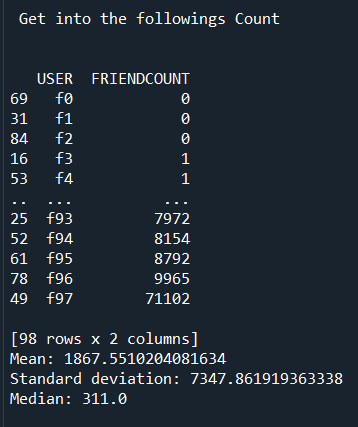
\includegraphics[trim=0 0 0 0, clip, width=\textwidth] {followings_consoleout.png}
    \caption{shows the console output for Q3}
    \label{fig:Running output}
\end{figure}

\subsection*{Discussion}
\emph{ For the major part Q3 followed samples for Q2, the major differences will only be listed.\\ \\}
\emph{I followed these instruction below:}
    \begin{itemize}
        \item I used the getUserFollowings function in line 138.
         \lstinputlisting[language=Python,caption=snapshot the getUserFollowings function used in  followerExtractor.py, label=Q1:import,firstnumber=138,firstline=138,lastline=138]{followerExtactor.py}
        \item This function used auth().friends on 98 instead of auth().followers\_ids, since it was retriving my following list
        \lstinputlisting[language=Python,caption=snapshot the getUserFollowings function used in  followerExtractor.py, label=Q1:import,firstnumber=94,firstline=94,lastline=94]{followerExtactor.py}
        \item The last difference is the friends following count instead of their followers\_count, in line 60 to 62
        \lstinputlisting[language=Python,caption=snapshot the getUserFollowings function used in  followerExtractor.py, label=Q1:import,firstnumber=60,firstline=60,lastline=62]{followerExtactor.py}
        \item Got values of: \\
                mean: 1867.55 followings\\
                std:7347.86\\
                median:311.0\\
        \item Comparing the mean of followings 1867.55 to my followings of 454  those that follow me have a higher followings than I do. 
    \end{itemize}
\section*{References}
\begin{itemize}
    \item {\url{https://stackabuse.com/rotate-axis-labels-in-matplotlib/}}
    \item {\url{https://www.youtube.com/watch?v=AYorFcI1MTU&t=212s}}

    
     \item {\url{http://jonathansoma.com/lede/foundations/classes/pandas\%20columns\%20and\%20functions/fixing-column-names-in-pandas/}}
     \item {\url{https://www.geeksforgeeks.org/python-tweepy-getting-the-number-of-followers-of-a-user/}}
     \item {\url{https://stackoverflow.com/questions/15943769/how-do-i-get-the-row-count-of-a-pandas-dataframe}}
     \item {\url{https://www.geeksforgeeks.org/python-user-object-in-tweepy/}}

\end{itemize}

\end{document}

